\subsection*{a. Borrar toda la información del cliente Paul Stevenson.}
Para esto usaremos la diferencia de conjuntos. Primero ubicaremos toda la información de Paul Stevenson en la tabla customers y posteriormente eliminaremos de la tabla.

Esto lo realizamos con la expresion:
\begin{equation}
\text{customer} - \sigma_{\text{customername} = \text{'Paul Stevenson'}} ( \text{customer} )
\end{equation}

Resultados obtenidos:
\begin{figure}[H]
  \centering
  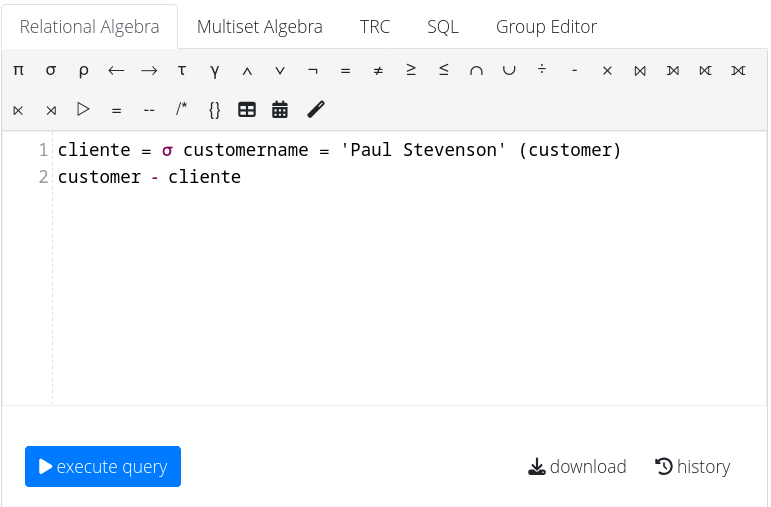
\includegraphics[width=0.7\textwidth]{imagenes/3.a-Query.png}
  \caption{Consulta}
\end{figure}

\begin{figure}[H]
  \centering
  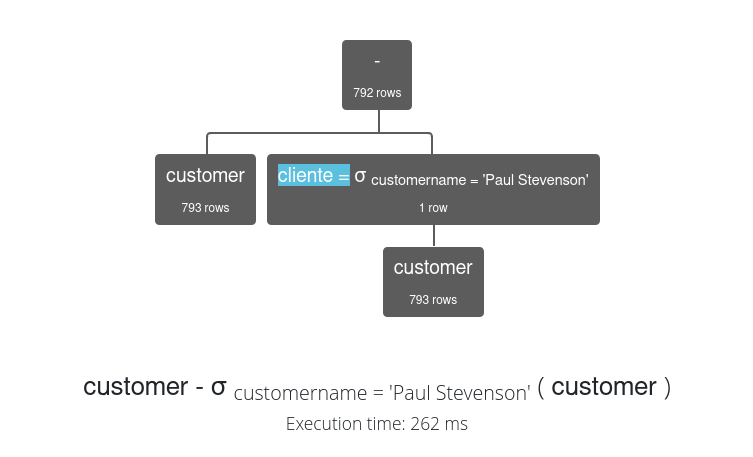
\includegraphics[width=0.7\textwidth]{imagenes/3.a-Three.png}
  \caption{Árbol de consulta.}
  \end{figure}
  
  \begin{figure}[H]
    \centering
    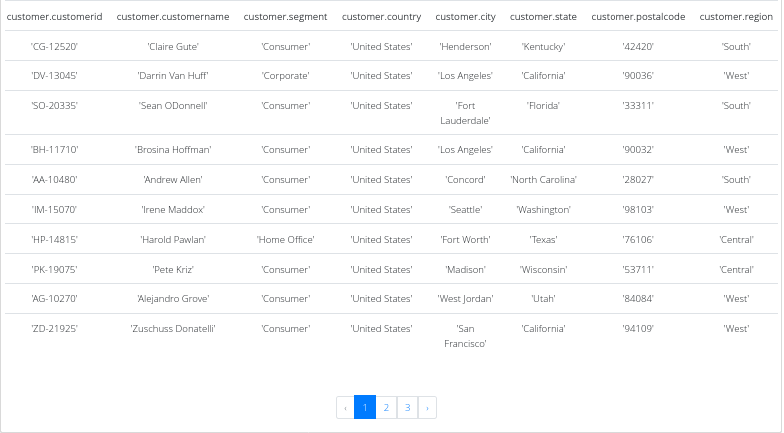
\includegraphics[width=0.7\textwidth]{imagenes/3.a-Tabla.png}
    \caption{Resultado de consulta.}
  \end{figure}
